\makeatletter
\setlength{\@fptop}{0pt}
\makeatother
\section[Simulation]{Simulation of Conservation laws}
\subsection{Trixi.jl}
\href{https://github.com/trixi-framework/Trixi.jl}{\ttfamily Trixi.jl} \cite{trixi} is a numerical simulation framework for conservation laws written in {\ttfamily Julia}. It is an open source package hosted on \href{https://www.github.com}{Github}
\subsection{Features of {\ttfamily Trixi.jl}}

{\ttfamily Trixi.jl} package can be used for simulation of conservation laws in $1$D, $2$D and $3$D and have the following features:
\begin{itemize}
    \item Support cartesian and curvilinear meshes.
    \item Structured and Unstructured meshes.
    \item AMR and Shock capturing.
    \item High-order accuracy in space and time.
    \item Discontinuous Galerkin methods.
    \item CFL-based and error-based time step control.
    \item Periodic and weakly-enforced boundary conditions.
\end{itemize}
{\ttfamily Trixi.jl} has multiple governing equations such as Compressible Euler, \linebreak Compressible Navier-Stokes, Shallow water equations etc. The code written in this package also have support for shared memory parallelization via multi-threading and multi-node parallelization via {\ttfamily Message Passing Interface (MPI)}. It also provides visualization and post-processing tools for the results.

It uses Runge-Kutta methods for discretization in time with other high-order methods for space discretization. RK methods are multi-stage methods for solving system of ODEs that we get after collocating the PDE at solution points, at the last step as described in the section of previous chapter \ref{step3}.

\section{{\ttfamily TrixiLW.jl}}
The one shortcoming of RK methods is their multi-stage nature. As we know, we need as many stages as the order of the method and sometimes number of stages has to be more than order of method to get the required accuracy in the case of high order methods. This can create a bottleneck in a parallel code as we need to communicate data at every stage and can significantly affect the performance of the code. 

In {\ttfamily TrixiLW}, we have extended the {\ttfamily Trixi} package to use Lax-Wendroff method for time discretization instead of RK methods. LW method is a single step update method. The features of {\ttfamily TrixiLW.jl} are as follows:

\subsection{Features of {\ttfamily TrixiLW}}
{\ttfamily TrixiLW} can be used for conservation laws in $2$D with the following features:
\begin{itemize}
    \item Support for cartesian and curvilinear meshes.
    \item Structured and Unstructured meshes.
    \item High-order accuracy in space and time.
    \item Discontinuous Galerkin methods.
    \item CFL-based and error-based time step control.
    \item Periodic and non-periodic boundary conditions.
    \item AMR and Shock capturing
\end{itemize}
This package also supports shared memory parallelization via multi-threading. As a part of this summer project, I have added support for multi-node parallelization via {\ttfamily Message Passing Interface (MPI)}. For visualization and post-processing, we use the tools of {\ttfamily Trixi} itself.

\subsection{Multi-node parallelization of {\ttfamily TrixiLW}}
Multi-node parallelization implies that we can use the computing units of \linebreak various nodes connected to each other via fast interconnects. This can help us encounter the issue of insufficient memory on a single node and harness the \linebreak computing power of many nodes. We can use memory of other nodes which are connected to each other via channel-based fabric such as {\ttfamily InfiniBand} that facilitates high-speed communication between interconnected nodes. 

Although, using multi-node parallelization can also creates a communication overhead for the running program yet it is used since there is a nice trade-off between the overhead created due to communication and other aspects such as memory, computing power, data storage etc. 

Message Passing Interface (MPI) is an open source implementation that laid down the rules of communication between processes. It is developed and maintained by \href{https://www.mpi-forum.org/}{MPI Forum}.
There are many open source libraries that are based on MPI and prvoide language specific routines. These includes {\ttfamily OpenMPI, MPICH} etc.

\subsubsection{Strategy of parallelization}
{\ttfamily TrixiLW.jl} is based on Lax-Wendroff Flux reconstruction (LWFR) method. In this method, we need to communicate $u$ (solution values), $U$ (time average solution) and $F$ (time average flux) values of the mpi\_interface elements to other required ranks.

\begin{figure}[!ht]
    \centering
    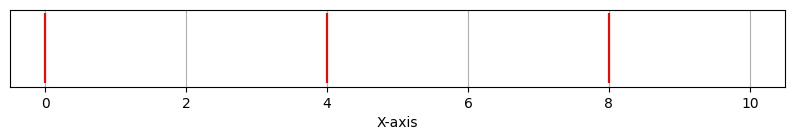
\includegraphics[width=0.9\linewidth]{attachments/1Dmesh.png}
    \caption{interfaces and mpi\_interfaces}
    \label{fig:1}
\end{figure}
For simplicity we are taking example of 1D mesh as in figure(\ref{fig:1}), the red lines are {\ttfamily mpi\_interfaces} which are not owned by the current rank and grey lines are {\ttfamily interfaces} which are owned by the current rank.
The values need to be communicated only at the {\ttfamily mpi\_interfaces}
and not at the normal {\ttfamily interfaces} as both the elements around normal {\ttfamily interfaces} are owned by the current rank. We have used non-blocking communication routines for communication between ranks. These routines include: {\ttfamily MPI\_Isend} and {\ttfamily MPI\_Irecv}.

\subsection{Data Structures}
At each interface, as we have seen, three variables needs to be stored $u$, $U$ and $F$, following is the {\ttfamily MPIInterfaceContainer} data structure that will be used to store the data.
\begin{listing}[!ht]
\centering
    \begin{minted}[linenos]{Julia}
# Container data structure (structure-of-arrays style) 
# for DG MPI interfaces
mutable struct MPIInterfaceContainerLW2D{uEltype <: Real}
                                        <:AbstractContainer
    u::Array{uEltype, 4}     # [leftright, variables, i, interfaces]
    U::Array{uEltype, 4}
    F::Array{uEltype, 4}
    local_neighbor_ids::Vector{Int} # [interfaces]
    orientations::Vector{Int}       # [interfaces]
    remote_sides::Vector{Int}       # [interfaces]
    # internal `resize!`able storage
    _u::Vector{uEltype}
    _U::Vector{uEltype}
    _F::Vector{uEltype}
end
    \end{minted}
    \caption{Struct for mpi\_interfaces}
    \label{list:1}
\end{listing}

The {\ttfamily struct} in listing (\ref{list:1}) has some extra fields for such as $\_u$, $\_U$ and $\_F$, these field are needed for internal storage since in {\ttfamily Julia} only 1D arrays can be resized.
Therefore, memory will be allocated for these 1D arrays and data will be stored in them. Later, that allocated memory will be re-used using {\ttfamily unsafe\_wrap} method of {\ttfamily Julia}
without making another copy of data hence avoiding unnecessary memory allocation.

Other field such as {\ttfamily local\_neighbor\_ids} will store {\ttfamily ranks} of neighboring interfaces, {\ttfamily orientations} will store the orientation of the interface (either x or y direction)
and {\ttfamily remote\_sides} will contain the information whether {\ttfamily mpi\_interfaces} are in positive direction or negative direction of the axis.

There will be another function called {\ttfamily prolong2mpiinterfaces!} which will be responsible for prolonging the element data to {\ttfamily mpi\_interfaces} and filling up the above mentioned container. After storing the element data in this container, we will be creating the buffers that will be used for MPI communication between ranks. The {\ttfamily MPICache} container will look something like this:
\begin{listing}[!ht]
    \centering
    \begin{minted}[linenos]{Julia}
mutable struct MPICache{uEltype <: Real}
    mpi_neighbor_ranks::Vector{Int}
    mpi_neighbor_interfaces::Vector{Vector{Int}}
    mpi_neighbor_mortars::Vector{Vector{Int}}
    # buffers for data storage
    mpi_send_buffers::Vector{Vector{uEltype}}
    mpi_recv_buffers::Vector{Vector{uEltype}}
    # requests object for non-blocking communication
    mpi_send_requests::Vector{MPI.Request}
    mpi_recv_requests::Vector{MPI.Request}
    n_elements_by_rank::OffsetArray{Int, 1, Array{Int, 1}}
    n_elements_global::Int
    first_element_global_id::Int
end
    \end{minted}
    \caption{Struct MPICache}
    \label{list:2}
\end{listing}

{\ttfamily mpi\_send\_buffers} and {\ttfamily mpi\_recv\_buffers} are a collection of buffers that store data for each rank present in communicator {\ttfamily MPI\_COMM\_WORLD}.

\subsection{Mesh Types: TreeMesh and P4estMesh}
In this project, the two types mesh structures used for discretization of domain for conservation laws are {\ttfamily TreeMesh} and {\ttfamily P4estMesh}. Each of these meshes have distinct properties and challenges involved in parallelization of code.

{\ttfamily TreeMesh} is a cartesian, $h$-non-conforming mesh type used in many parts of of {\ttfamily TrixiLW.jl}. Often, the support for this mesh type is developed best for serial and parallel code since it was the first mesh type in {\ttfamily TrixiLW.jl}, and it is available in two spatial dimensions for both serial and parallel code. It is limited to hypercube domain i.e. squares in 2D.

{\ttfamily P4estMesh} is a unstructured, curvilinear, non-conforming mesh used in {\ttfamily TrixiLW.jl}. It is available for two spatial dimensions with quadrilateral 2D cells. Parallel code for this mesh have also been developed.
\begin{figure}[!ht]
    \centering
    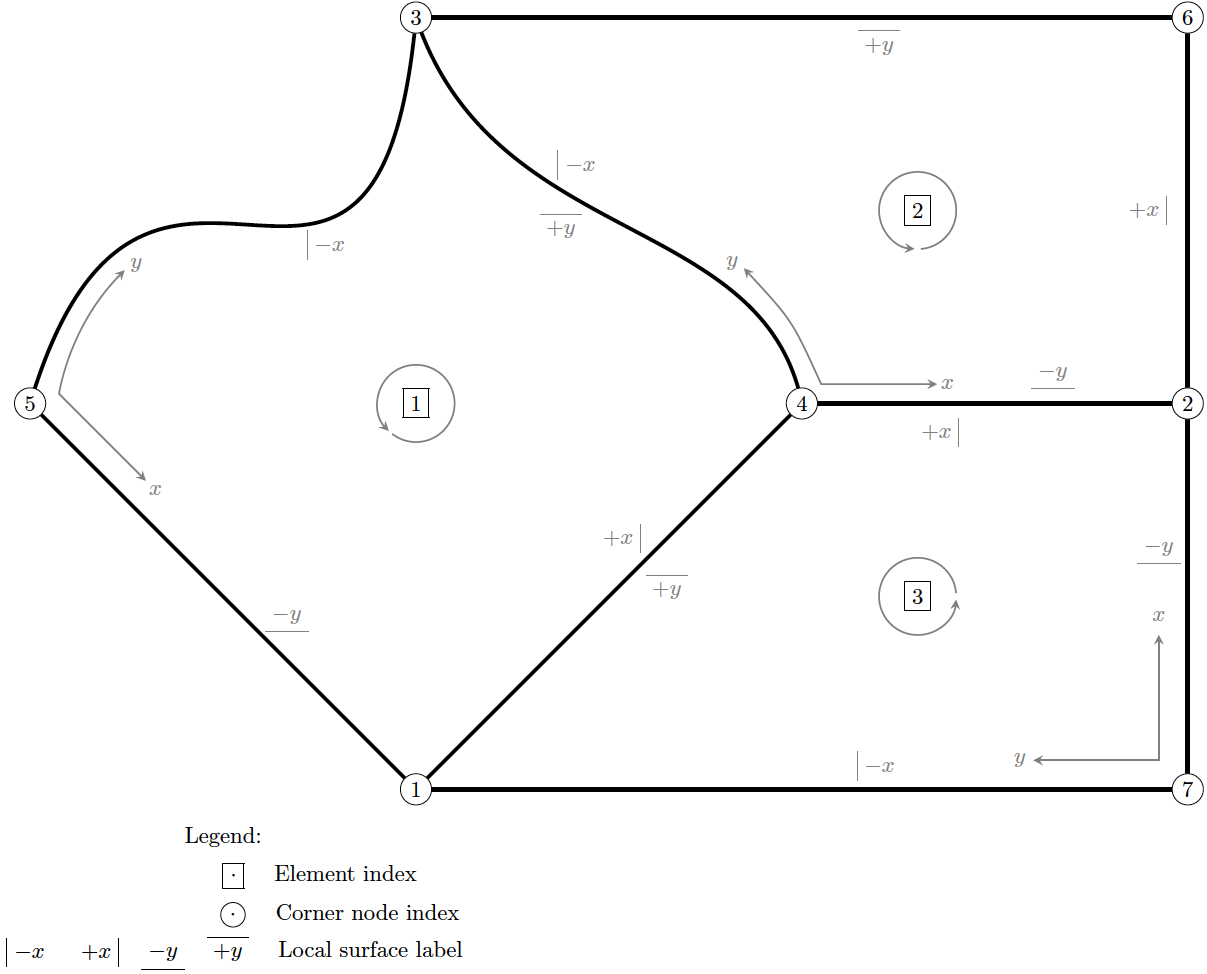
\includegraphics[width=0.80\linewidth]{attachments/p4estmesh.png}
    \caption{P4est Mesh}
    \label{fig:4.2}
\end{figure}

The figure(\ref{fig:4.2}) shows the two-dimensional unstructured curved mesh with 3 elements and the data that needs to be stored in order to navigate through the mesh. We have extended {\ttfamily Trixi.jl} to support Lax-Wendroff flux reconstruction (LWFR) method hence our main goal was to write code that can re-use most of the functionality provided by {\ttfamily Trixi.jl} and only the code required by LWFR part should be written again.

All the functions that are exclusive to LWFR are dispatched with a extra argument {\ttfamily time\_discretization} which is of type {\ttfamily AbstractLWTimeDiscretization} in order to differentiate these functions. In the next section, we will discuss an alternative approach to parallelization than using non-blocking communication routines such as {\ttfamily MPI\_Isend} and {\ttfamily MPI\_Irecv}. 

\begin{center}
    \rule{3cm}{1pt}
\end{center}